
\documentclass[paper=a4, fontsize=11pt]{scrartcl} % A4 paper and 11pt font size

\usepackage[T1]{fontenc} % Use 8-bit encoding that has 256 glyphs
\usepackage{fourier} % Use the Adobe Utopia font for the document - comment this line to return to the LaTeX default
\usepackage[english]{babel} % English language/hyphenation
\usepackage{amsmath,amsfonts,amsthm} % Math packages
\usepackage{wrapfig}
\usepackage{lipsum} % Used for inserting dummy 'Lorem ipsum' text into the template
\usepackage{tikz}
\usepackage{amsmath}
\usepackage{sectsty} % Allows customizing section commands
\allsectionsfont{\centering \normalfont\scshape} % Make all sections centered, the default font and small caps

\usepackage{fancyhdr} % Custom headers and footers
\pagestyle{fancyplain} % Makes all pages in the document conform to the custom headers and footers
\fancyhead{} % No page header - if you want one, create it in the same way as the footers below
\fancyfoot[L]{} % Empty left footer
\fancyfoot[C]{} % Empty center footer
\fancyfoot[R]{\thepage} % Page numbering for right footer
\renewcommand{\headrulewidth}{0pt} % Remove header underlines
\renewcommand{\footrulewidth}{0pt} % Remove footer underlines
\setlength{\headheight}{4pt} % Customize the height of the header
\usepackage{float}
\numberwithin{equation}{section} % Number equations within sections (i.e. 1.1, 1.2, 2.1, 2.2 instead of 1, 2, 3, 4)
\numberwithin{figure}{section} % Number figures within sections (i.e. 1.1, 1.2, 2.1, 2.2 instead of 1, 2, 3, 4)
\numberwithin{table}{section} % Number tables within sections (i.e. 1.1, 1.2, 2.1, 2.2 instead of 1, 2, 3, 4)

\setlength\parindent{0pt} % Removes all indentation from paragraphs - comment this line for an assignment with lots of text

%----------------------------------------------------------------------------------------
%	TITLE SECTION
%----------------------------------------------------------------------------------------

\newcommand{\horrule}[1]{\rule{\linewidth}{#1}} % Create horizontal rule command with 1 argument of height

\title{	
\normalfont \normalsize  % Your university, school and/or department name(s)
\horrule{0.5pt} \\[0.4cm] % Thin top horizontal rule
\huge Physics 422 H.W. 1\\ % The assignment title
\horrule{2pt} \\[0.5cm] % Thick bottom horizontal rule
}

\author{Josh Lucas} % Your name

\date{\normalsize\today} % Today's date or a custom date

\begin{document}

\maketitle % Print the title

%----------------------------------------------------------------------------------------
%	PROBLEM 1
%----------------------------------------------------------------------------------------

\section{Lattice Cells and Basis}
\textbf{Consider the pattern and indicate the following: A \textbf{Rectangular unit cell}, a \textbf{Primitive unit cell}, and the \textbf{Basis} of this "crystal."}\\
\begin{wrapfigure}[20]{l}{0.55\textwidth}
\includegraphics[width=8cm]{Lattice}
\caption{2-D Lattice from bottom to top: Primitive cell, Retangular cell}
\end{wrapfigure}\\
We can place the \textbf{rectangular cell} around the top two rows, if stacked on top of each other they will form the pattern of atoms repeatedly.\\ The rectangular cell is not the smallest volume comprising all of the atoms, the \textbf{primitive unit cell} is the smallest volume containing all points and can be formed by diagonal lines at a relative angle of $\frac{\pi}{2}$ to each other. With this primitive unit cell we can repeat the pattern with only one instance of each particle.\\
The \textbf{Basis} consists of four particles. If considering the origin to be the bottom left particle and disregarding the tilt of the axes we can say the basis is 
\begin{equation*}
basis = \begin{cases} \odot\  & @ (0,0) \\ \bigcirc , & @ (\frac{1}{8},0) \\ \diamond & @ (0,\frac{1}{2}) \\ \oplus &  @(\frac{1}{8},\frac{1}{2}) \end{cases}
\end{equation*} 

If the axes are taken into account with the corner at the origin the basis becomes,
\begin{equation*}
 = \begin{cases} \odot\  & @ (\frac{1}{8},\frac{1}{4}) \\ \bigcirc  & @ (\frac{1}{4},\frac{1}{8}) \\ \diamond & @ (\frac{3}{4},\frac{7}{8}) \\ \oplus &  @(\frac{7}{8},\frac{3}{4}) \end{cases}
\end{equation*} 



%\begin{tikzpicture}
%  %\draw[thin,gray!40] (-2,-2) grid (2,2);
%  %\draw[<->] (-2,0)--(2,0) node[right]{$x$};
% % \draw[<->] (0,-2)--(0,2) node[above]{$Z$};
%  \draw[line width=2pt,red,-stealth](0,0)--(6,0) node[anchor=south west]{$\boldsymbol{\vec{a_1}}$};
%  \draw[line width=2pt,red,-stealth](6,0)--(6,2) node[anchor=north east]{$\boldsymbol{\vec{a_2}}$};
%    \draw[line width=2pt,black,-stealth](0,2)--(6,2) node[anchor=south west]{};
%  \draw[line width=2pt,black,-stealth](0,0)--(0,2) node[anchor=north east]{};
%\end{tikzpicture}
%\hspace{25mm}
%\begin{tikzpicture}
%  %\draw[thin,gray!40] (-2,-2) grid (2,2);
%  %\draw[<->] (-2,0)--(2,0) node[right]{$x$};
% % \draw[<->] (0,-2)--(0,2) node[above]{$Z$};
%  \draw[line width=2pt,red,-stealth](0,0)--(1,1) node[anchor=north west]{$\boldsymbol{\vec{a_1}}$};
%  \draw[line width=2pt,red,-stealth](1,1)--(0,2) node[anchor=north east]{};
%   \draw[line width=2pt,black,-stealth](0,2)--(1,3) node[anchor= east]{};
%  \draw[line width=2pt,black,-stealth](1,1)--(2,2) node[anchor=north west]{};
%   \draw[line width=2pt,black,-stealth](2,2)--(1,3) node[anchor= west]{};
%\end{tikzpicture}

\section{Nearest Neighbors}
%------------------------------------------------
\textbf{a) What are the number of nearest neighbors to each lattice point in the simple cubic, BCC, and FCC latices?}
\\
\\
\textbf{Simple Cubic }$\bullet$ In the simple cubic lattice the atom has four neighbors in the horizontal plane and a neighbor above and below giving it a \textbf{coordination number of 6}.
\newline
\textbf{Body-Centered Cubic}$\bullet$ In the body-centered cubic, BCC, the atom at the center has four  neighbors above and four below giving it a \textbf{coordination number of 8.}\\
\textbf{Face-Centered Cubic}$\bullet$  The face centered cubic has an atom centered on each face with nearests neighbors located ad the 8 other adjacent faces as well as the four corners of the atom's face giving it a \textbf{coordination number of 12.}
\newline \\
\textbf{b)  If the conventional unit cell has sides of length $a_1$, what are the distances between nearest neighbors in each case?}
\\
\textbf{Simple Cubic }$\bullet$  The distance to the nearest neighbor in the simple cubic is the length of the primitive vector $a_1$ with a magnitude of a.\\
\textbf{Body-Centered Cubic}$\bullet$  The body-centered cubic has an atom at the center of the cube with equal distance to the eight corners. The vector from a corner at the origin to the center of the cube is $$\vec{r} = \frac{1}{2} (a_1+a_2+a_3)$$  making the nearest atom's distance the magnitude of the vector,
\begin{equation*}
\bigg|\frac{1}{2} (a_1+a_2+a_3)\bigg| = \sqrt{\frac{1}{2}a_1^2+\frac{1}{2}a_2^2+\frac{1}{2}a_3^2 } = \sqrt{\frac{3}{4}a^2} = \frac{a}{2}\sqrt{3}
\end{equation*}
The distance to the nearest neighbor in the body centered cubic is $\frac{a}{2}\sqrt{3}$ \\

\textbf{Face-Centered Cubic}$\bullet$  The face-centered cubic is more densely packed than the BCC. the nearest neighbor will always be $\frac{1}{2}a$ in two orthogonal directions and in the same plane as another, such as,

$$\vec{r} =  \frac{1}{2}\vec{a_x} +\frac{1}{2}\vec{a_y} + (0)\vec{a_z}$$ 
or
$$\vec{r} =  (0)\vec{a_x} +\frac{1}{2}\vec{a_y} + \frac{1}{2}\vec{a_z}$$ 
 making the nearest atoms distance the magnitude
\begin{equation*}
\bigg| \frac{1}{2}\vec{a_x}+\frac{1}{2}\vec{a_y}\bigg| = \sqrt{(\frac{1}{2}a_x)^2+(\frac{1}{2}a_y^)2 } = \sqrt{\frac{1}{2}a^2} = \frac{a}{2}\sqrt{2}
\end{equation*}
The distance to the nearest neighbor in the body centered cubic is $\frac{a}{2}\sqrt{2}$ \\


\section{Zincblende}
\textbf{Considering the figure:} \\
\textbf{a) What is the Bravais Lattice type?}\\
The lattice type is a \textbf{face center cubic} with four lattice points per unit cell. The individual lattice points form a tetrahedral structure consisting of four Zn atoms and one S atom.



\textbf{b) Describe the basis.}\\
The basis consists of four Zn atoms and  a single S atom connected in a tetrahedral structure with four lattice points per unit cell. Starting with origin at the bottom left corner of the unit cell the basis's additional Zinc atoms are the front face, bottom face and left face with the S atom at the center.
\begin{figure}[h]
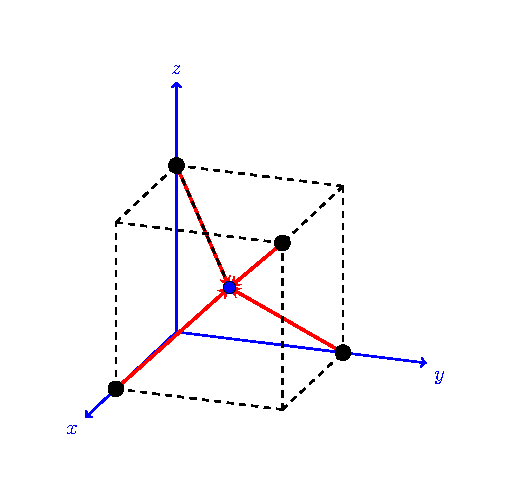
\includegraphics[width=7cm]{ZnS}
\caption{Basis of Zincblende showing tetrahedral structure}
\end{figure}

\begin{figure}[h]
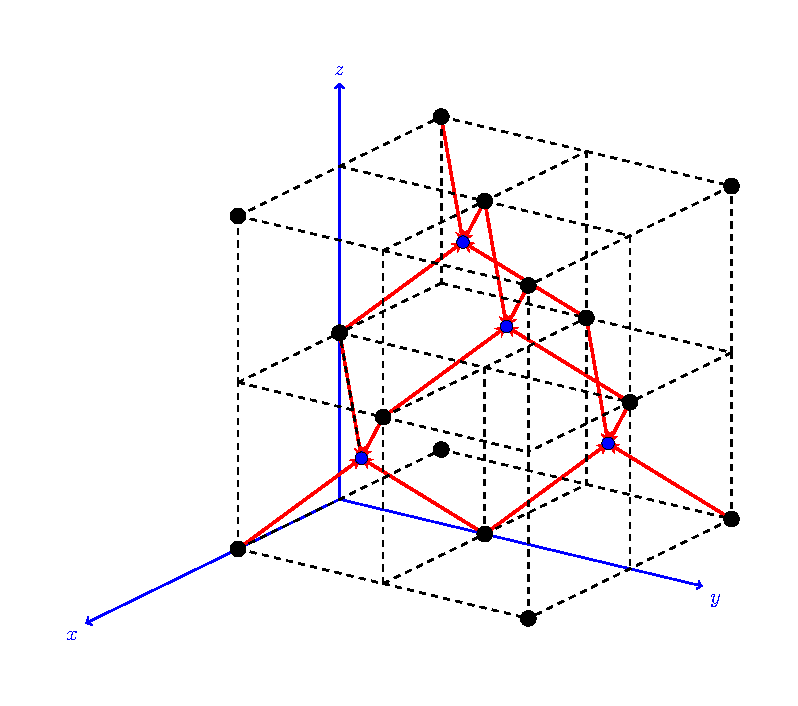
\includegraphics[width=7cm]{ZnSUnit}
\caption{Expanded structure of unit cell}
\end{figure}
\begin{equation*}
Basis = \begin{cases} Zn_1  & @ (0,0,0) \\ 
 Zn_2  & @ (\frac{1}{2},0,\frac{1}{2})\\
 Zn_3 & @ (\frac{1}{2},\frac{1}{2},0) \\
 Zn_4 & @ (0,\frac{1}{2},\frac{1}{2})\\
 S & @ (\frac{1}{4}, \frac{1}{4}, \frac{1}{4}) \end{cases}
\end{equation*} 

 
\vspace{5mm}

\textbf{c)  Given that a = 0.541 nm, calculate the nearest neighbor Zn-Zn, Zn-S, and S-S distances.}


\textbf{Zn - Zn }$\bullet$ The vector from a Zn atom to another is the face-centered vector with a magnitude of, 
$$a \frac{\sqrt{2}}{2} \rightarrow (0.541nm)\frac{\sqrt{2}}{2} = 3.82\AA$$
The distance from a Zn atom to another Zn atom is $3.82\AA$\\

\textbf{Zn - S} $\bullet$ From a Zn atom located at the origin on a face to a S atom the vector would be a quarter of a in each direction,
\begin{equation*}
\text{Zn-S} = \vec{r} = \frac{1}{4}(\vec{a_x}+\vec{a_y}+\vec{a_z})
\end{equation*}
Where the magnitude is,
\begin{equation*}
\sqrt{(\frac{1}{4}a)^2}= \sqrt{\frac{3}{16}a^2} = \frac{\sqrt{3}}{4} a \rightarrow \frac{\sqrt{3}}{4}\ (.541 nm) = 2.34\AA
\end{equation*}
 The distance from a Zn atom to a S atom is 2.34\AA \\
 
\textbf{S - S} $ \bullet$ The distance from the center of an S atom to another S atom is the same as the Zn to Zn which is,  $a\frac{\sqrt{2}}{2} = (0.541nm)\frac{\sqrt{2}}{2} = 3.82\AA$
 
\section{Packing Fraction}
\textbf{Imagine a FCC lattice with a one atom basis. Determine the packing fraction of this crystal by modeling the atoms as hard spheres that touch their nearest neighbors.}\\

The packing efficiency is equivalent to the volume of the atoms in the unit cell per total volume of the unit cell multiplied by 100.
\begin{equation*}
\text{Packing Efficiency} = \frac{\text{Volume}_{\text{Atoms  in  unit cell}}}{\text{Volume}_{\text{unit cell}}} \times 100
\end{equation*}

\begin{figure}[h]
\includegraphics[width=10cm]{bcc}
\centering
\caption{Face Centered Cubic showing the truncated atoms in the unit cell}
\end{figure}

 To find the volume of the cell we need to find the lengths of the sides. The four corner atoms are themselves only a quarter inside the cell, with the face atom half in the cell, but along the full diameter. The bottom corner to top corner angle is $\frac{\pi}{4}$ as seen in figure 4.1, so we can then solve for the length of sides using the Pythagorean theorem or trigonometric relations,
 \begin{equation*}
 b = \frac{1}{2}r + 2r + \frac{1}{2}r = 4r
 \end{equation*}
\begin{equation*} 
\begin{split}
b \cos{\theta} & = l \\
 4r \cos{\frac{\pi}{4}}& = l \\
 4r(\frac{\sqrt{2}}{2}) & = l \\
 2\sqrt{2} r & = l \\
\end{split}
\end{equation*}
The sides extend in to three dimensions making the volume of the unit cell $l^3$,
\begin{equation*}
l^3 = (2\sqrt{2}r)^3 = 16 \sqrt{2} r^3
\end{equation*}




We know that there is a total of four atoms contained in a FCC unit cell, two from the half atoms at the faces and 2 from the quartered corners. The volume of the sphere is $\frac{4 \pi r^3}{3}$, multiplying the volume by four atoms,
\begin{equation*}
Volume_{Atoms} = 4\ atoms\ (\frac{4 \pi r^3}{3}) = \frac{16 \pi r^3}{3} 
\end{equation*}

When we divide by the total volume of the unit cell and multiply by 100 we have,
\begin{equation*}
\text{Packing Efficiency} = \frac{\text{Volume}_{\text{Atoms  in  unit cell}}}{\text{Volume}_{\text{unit cell}}} \times 100 = \frac{\frac{16 \pi r^3}{3} }{16\sqrt{2}\ r^3 } = \frac{\pi}{3\sqrt{2}} \times 100 = 74 \% 
\end{equation*}

The \textbf{Face Centered Cubic} when confined to only one type of atom has a packing efficiency of approximately $74\%$.
%----------------------------------------------------------------------------------------

\end{document}